\section{Problem no.1}

Here is presented the design of a corporate beam forming network. By specification, FR4 is given as substrate (the technological specifications follow in table 1).

 \begin{table} [b]
 	\label{tab:p1_FR4}
 	\caption{FR4 technological specifications.}
 	\centering	
 	\begin{tabular}{lrrr} 
 		\toprule 
 		Quantity & Symbol & value & \\
 		\midrule
		Dielectric permittivity &$\epsilon_{r}$		&4.3		& 		\\
 		Substrate height&	h				& 1.5		&  mm	\\ 
 		Metal thickness&t	& 0.1	& mm\\
 		Minimum strip width &W\textsubscript{min}&0.15 & mm \\
 		Minimum spacing between lines &$\Delta$s\textsubscript{min}&0.175 & mm \\
 		\bottomrule 
 	\end{tabular}	
 \end{table}

The antenna's radiating part requires four radiators with cosine-over-pedestal tapering, hence the BFN is symmetric with respect to the feeding line. 

\begin{figure}[t] 
	\centering
	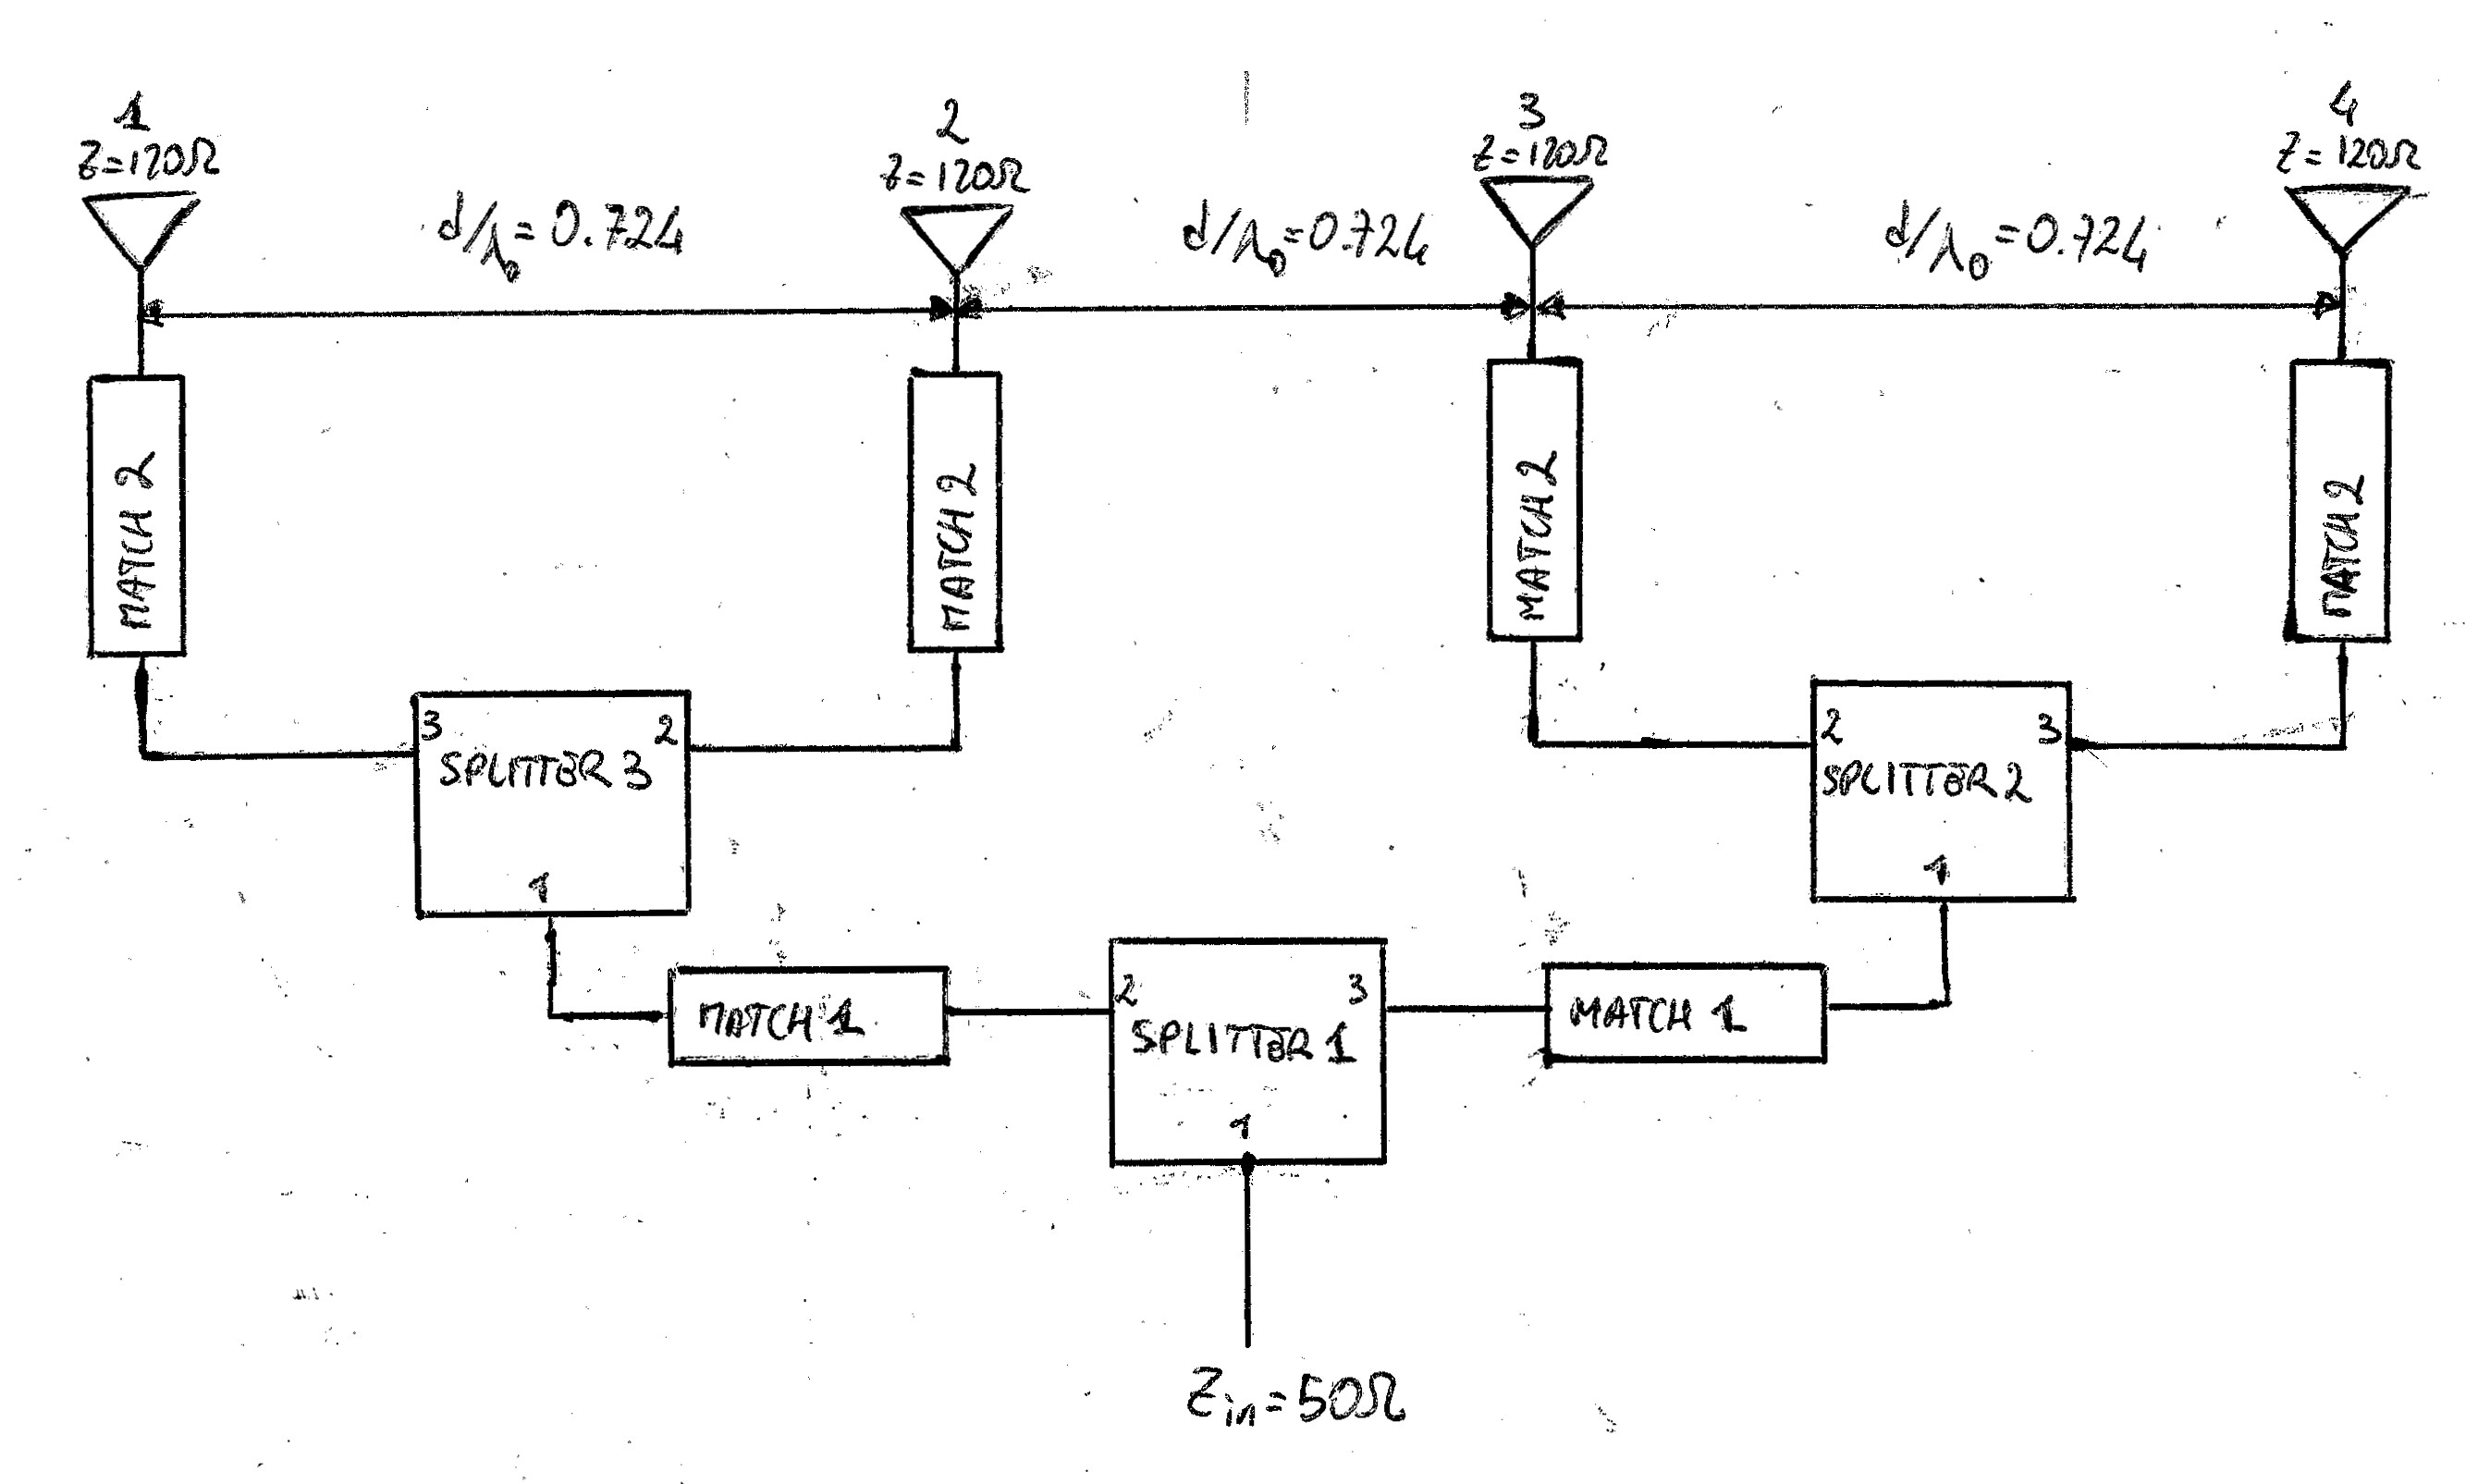
\includegraphics[scale=0.5]{p1_bfn_block}
	\caption{Beam forming network's block diagram.}
	\label{fig:p1_bfn_block}
\end{figure}

One possible implementation is proposed in figure \ref{fig:p1_bfn_block}, where the building blocks can be identified as follows: 
\begin{description}
	\item [Splitter1] this section matches the input line to Z\textsubscript{in}=50$\Omega$ at the input port. Moreover, it evenly splits the power into two branches that follows, therefore this is a 3dB splitter. 
	\item [Splitter2] this section matches the radiating elements with section1 outputs, moreover it convey power into the radiators giving the correct power ratio between elements.
	\item [Splitter3] this is symmetric to section2 with respect to the feeding line longitudinal axis. 
	\item [Match1] these lines acts as matching connection from power splitter1 to power splitters2 and 3, moreover they are used to adjust the distance between elements.
	\item [Match2] matching connections between radiators and power splitters2,3;
\end{description}
Overall the BFN should be designed in order to be compliant with the requirement on:
\begin{itemize}
	\item grating lobes, related to the element spacing d (d/$\lambda_0=0.724$);
	\item amplitude tapering between edge and centre elements;
	\item main beam direction: since the array is broadside then the phase shift among elements must be null.
\end{itemize}
Another requirement concerns the full array's dimensions, although those are not specified particular attention will be devoted into taking the minimal amount of space.
Each block's design and simulation are reported in the following paragraphs.

\subsection{Splitter 1 design}
Figure \ref{fig:p1_sec1_block} shows the block diagram of splitter1. 
\begin{figure}[H] 
	\centering
	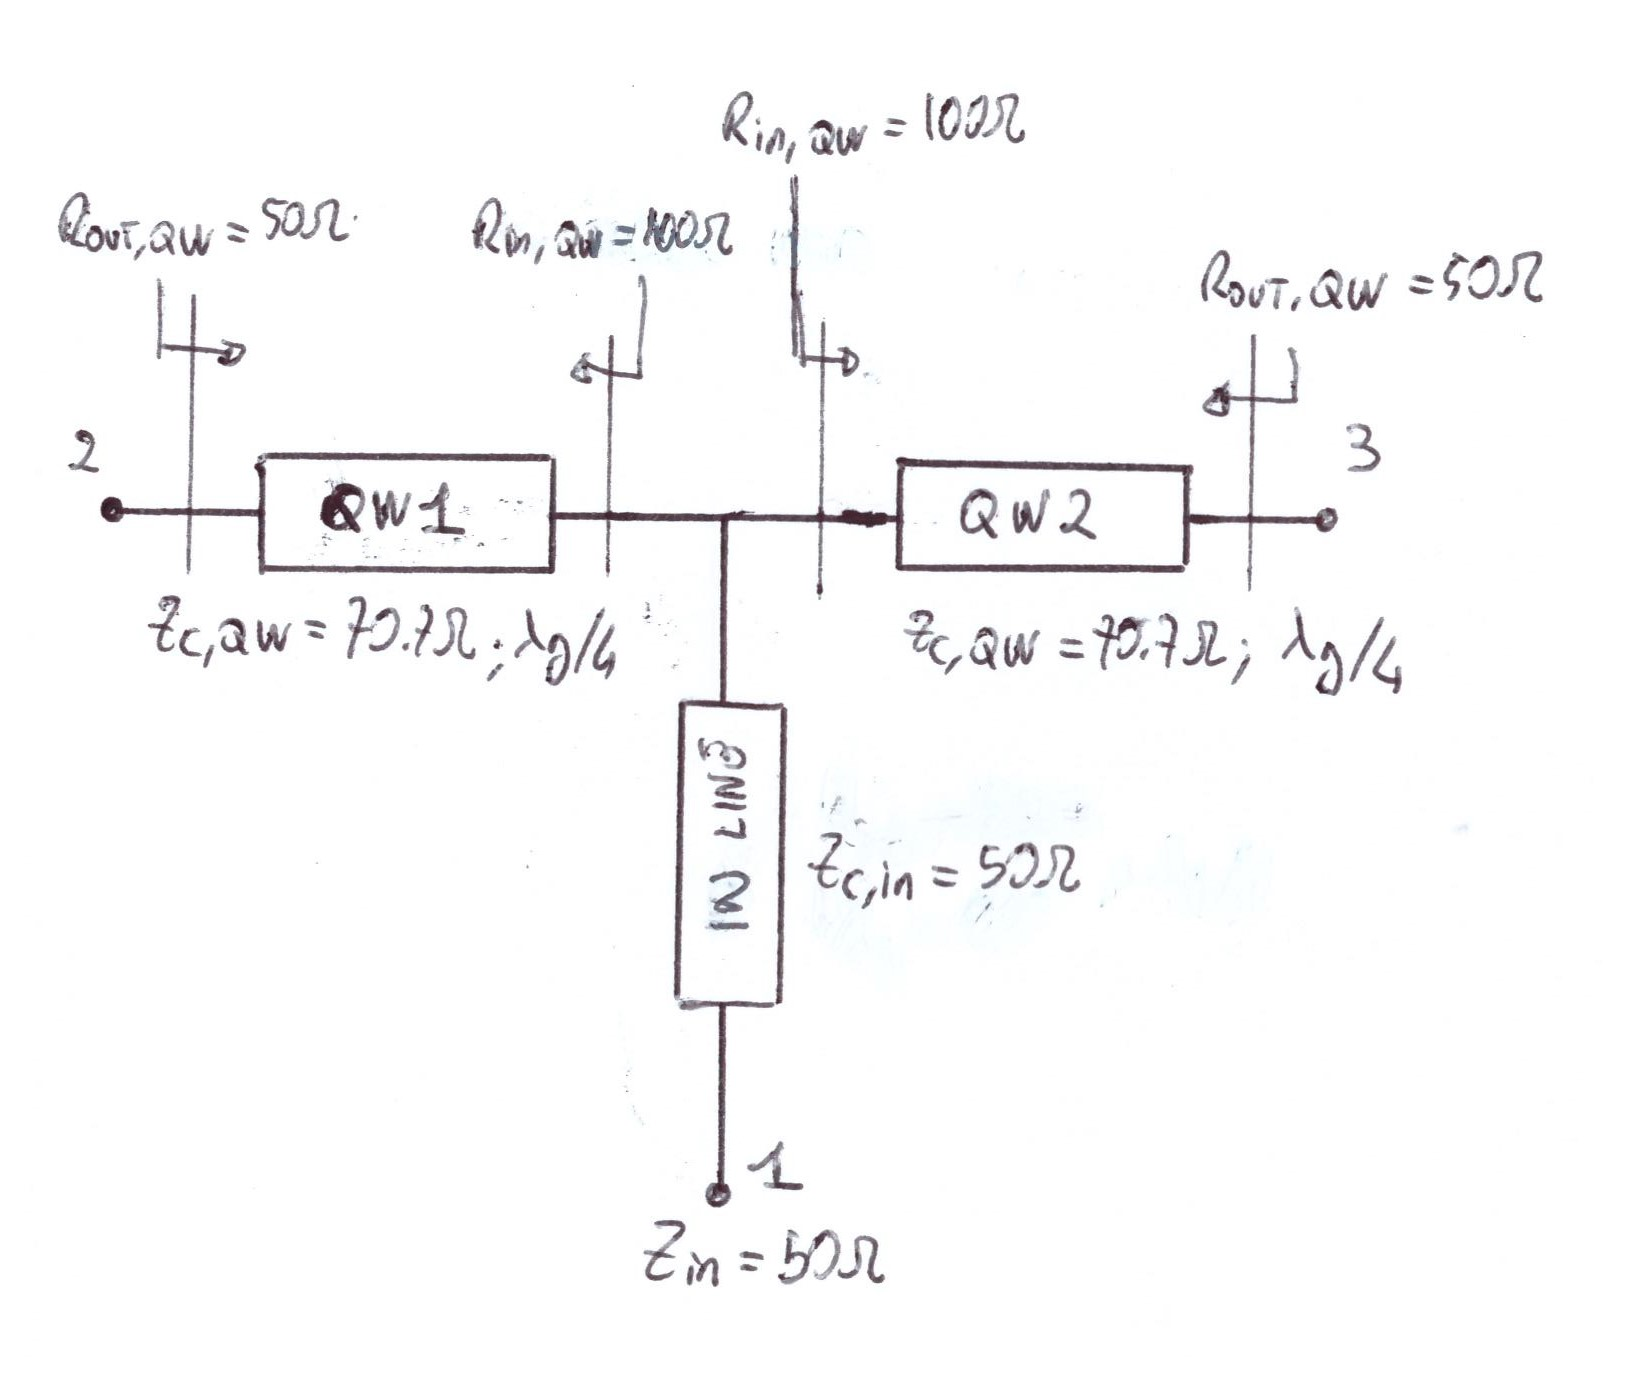
\includegraphics[scale=0.5]{p1_sec1_bl}
	\caption{Splitter1 TXL implementation. }
	\label{fig:p1_sec1_block}
\end{figure}
The input line is power matched to the input port by means of a 50$\Omega$ line whose length has been chosen arbitrarily. To evenly split the power into port 2 and 3 we use a T-junction made up of two quarter-wavelength transformers. This components show real input and output impedance and the following relation for their characteristic impedance holds:
\begin{equation}
	\label{eq:p1_ZcQW}
	Z_{c,QW} =R_{c,QW}=\frac{1}{G_{c,QW}}= \sqrt{R_{in,QW}\cdot R_{out,QW}} 
\end{equation}
As a first approximation, the two quarter-wavelength transformers are seen as two parallel admittances from the input port, then to have the 50$\Omega$ matching we have:
\begin{equation}
	G_{c,QW1}+G_{c,QW2}=\frac{1}{Z_{in}}=\frac{1}{50\Omega} \; \Rightarrow \; Z_{c,QW1}=Z_{c,QW2}=Z_{c,QW}=100\Omega \notag
\end{equation}
 Willing to reduce impedance discontinuities within the network, the section's output impedance is set to 50$\Omega$ too, hence:
\begin{equation}
	Z_{c,QW}= \sqrt{R_{in,QW}\cdot R_{out,QW}}=\sqrt{100\Omega\cdot 50\Omega}=70.7\Omega \notag
\end{equation}
\begin{figure}[t] 
	\centering
	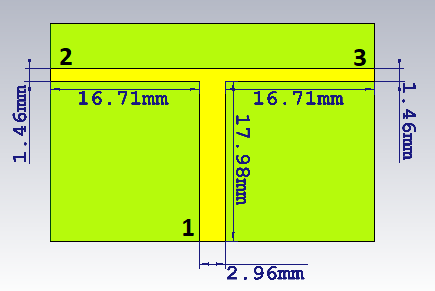
\includegraphics[scale=0.5]{p1_sec1_ustrip}
	\caption{Splitter1 microstrip implementation. }
	\label{fig:p1_sec1_ustrip}
\end{figure}
Finally the design has been converted from ideal microstrip lines to physical lines by means of TX-LINE: Transmission Line Calculator (from NI AWR Design Environment) and eventually implemented in CST DS\texttrademark{} for the optimization process. 
Theoretical and optimized dimensions are reported in table 2 and 3. The resulting scattering parameters are shown in figure \ref{fig:p1_sec1Scatt}: both power splitting and phase behaves as expected. Figure \ref{fig:p1_sec1_ustrip} depicts the microstrip implementation of this section.
\begin{table} [H]
	\label{tab:p1_sec1DimIN}
	\caption{Splitter1: Input line dimensions}
	\centering	
	\begin{tabular}{lccc} 
		\toprule
			& theoretical & optimized&\\
		\midrule 
		W\textsubscript{in} 	&	3.02		&	2.91	 & mm 		\\
		Z\textsubscript{c,in}	& 	50 			& 50.06		&$\Omega$ \\
		\bottomrule
	\end{tabular}	
\end{table}
\begin{table} [H]
	\label{tab:p1_sec1DimQW}
	\caption{Splitter1: quarter-wavelength transformer dimensions}
	\centering	
	\begin{tabular}{lccc} 
		\toprule
		& theoretical & optimized&\\
		\midrule 
		W\textsubscript{QW} 	&	1.59		&	1.49	& mm		\\
		L\textsubscript{QW}	&	17.25		& 	17.3		& mm	\\ 
		Z\textsubscript{c,QW}& 	70.7 &73.1	&$\Omega$ \\
		\bottomrule
	\end{tabular}	
\end{table}
\begin{figure}[p] 
	\centering
	\subfloat[][\emph{Modulus}]{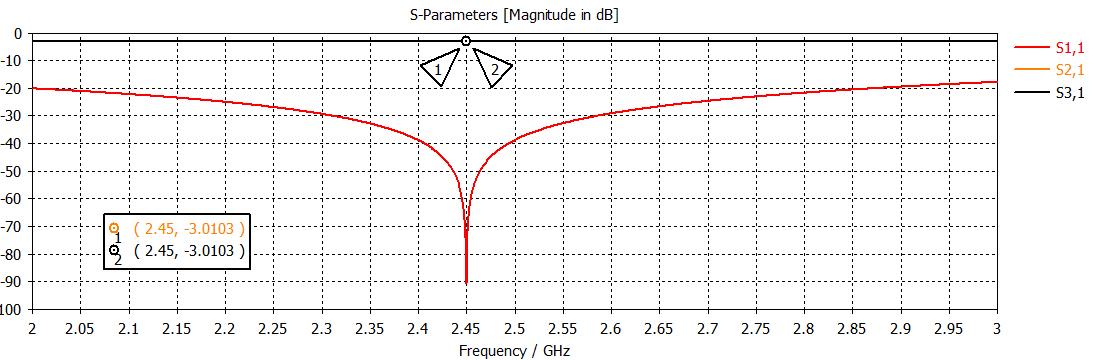
\includegraphics[scale=.6,angle=90]{p1_sec1_Smod}}\quad
	\subfloat[][\emph{Phase}]{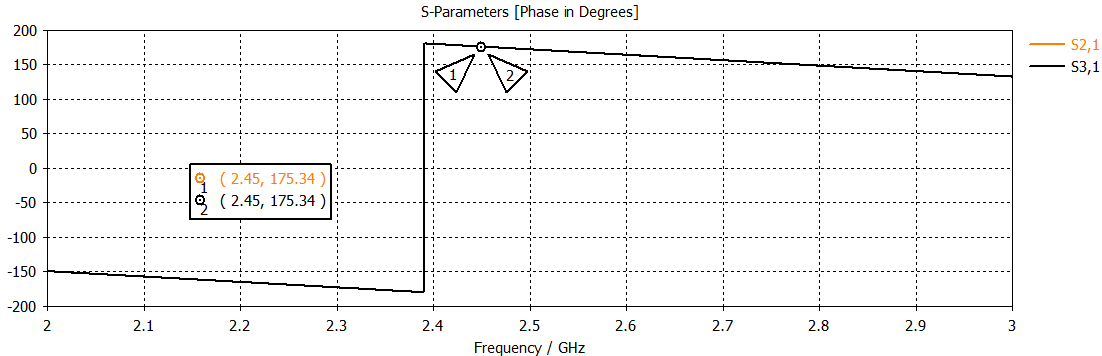
\includegraphics[scale=.6,angle=90]{p1_sec1_Sph}}\\
	\caption{Section 1 most important scattering parameters. As it appears both input matching and even power splitting are accomplished, the phase shift is null (reference impedance 50$\Omega$).}
	\label{fig:p1_sec1Scatt}
\end{figure}
\newpage

\subsection{Splitters2,3 and match2 design}

Figure \ref{fig:p1_sec2_block} shows the block diagram of splitter2 and match1 (splitter3  is specular).
\begin{figure}[H] 
	\centering
	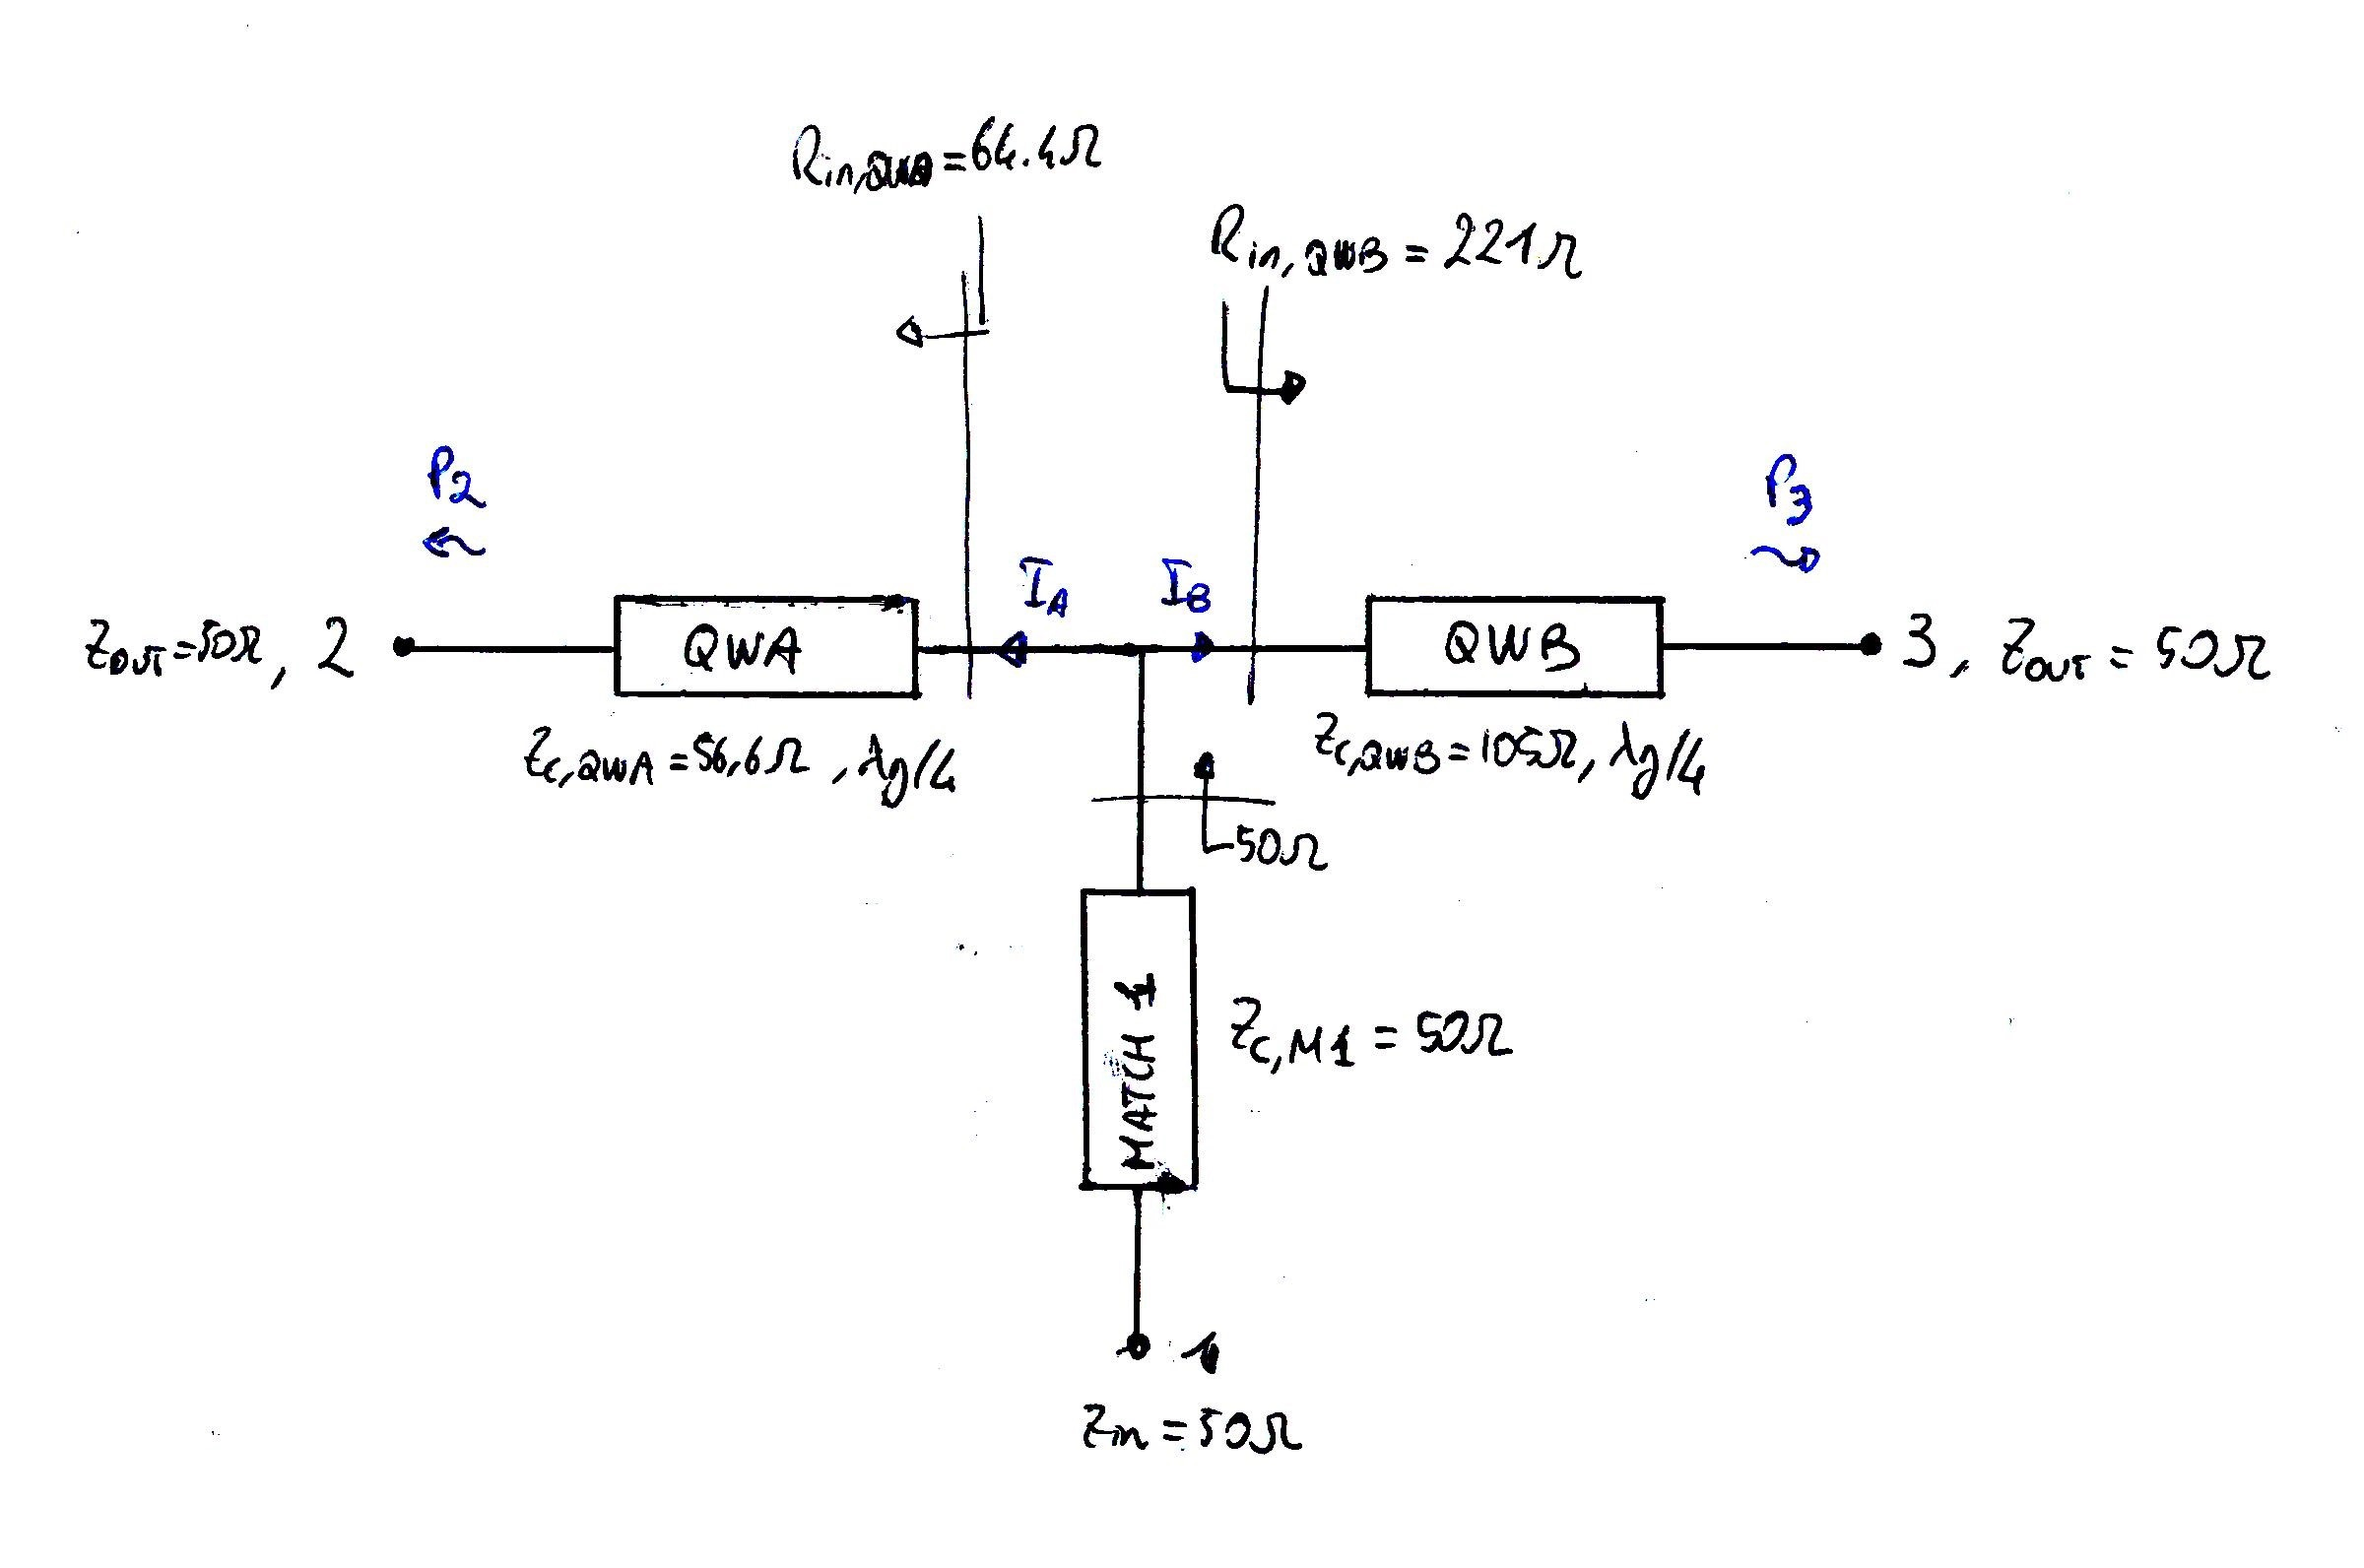
\includegraphics[scale=0.5]{p1_sec2_block}
	\caption{Splitter2 and match1 TXL implementation. }
	\label{fig:p1_sec2_block}
\end{figure}
Match1 is designed as, 50$\Omega$ characteristic impedance line. Since both the output of splitter1 and the input of splitter2,3 are matched to 50$\Omega$, the length of these line can be chosen as necessary to impose the correct distance between the radiators. Again, splitter2,3's output impedance is set to Z\textsubscript{out}=50$\Omega$ to avoid abrupt mismatch in contiguous lines connections. Moreover, imposing Z\textsubscript{in}=50$\Omega$ we also avoid the appearance of lines narrower than W\textsubscript{min} within the two splitters.

Again, quarter-wavelength transformers are employed to provide the correct current tapering for the radiators, this time they act as uneven power divider. To design that we will consider the power entering and exiting the component.
Having chosen as tapering t=0.54, then:
\begin{equation}
	\frac{S_{31}}{S_{21}}=0.54 \; \Rightarrow \; \frac{P_3}{P_2}=\Bigg(\frac{S_{31}}{S_{21}}\Bigg)^2=0.292 \Rightarrow \frac{P_3}{P_2}=-5.34dB \notag
\end{equation} 
where S\textsubscript{21} and S\textsubscript{31} are the scattering transmission coefficients at port 2 and 3. In particular P\textsubscript{2} is the power exiting the splitter and directed to the centre element, whereas P\textsubscript{3} goes to the edge radiator (supposing lossless TXL):
\begin{equation}
	\begin{cases}
		P_2 = P_a = \frac{1}{2}R_{in,QWa}|I_A|^2 \notag \\	
		P_3 = P_b = \frac{1}{2}R_{in,QWb}|I_B|^2 \notag	
	\end{cases}	
\end{equation}
As before, the two impedance transformers are seen as two in-parallel conductances from port 1, then the following system holds: 
\begin{equation}
	\begin{cases} 
		\frac{1}{R_{in,QWa}}+\frac{1}{R_{in,QWb}}=\frac{1}{Z_{in}} \notag\\
		\frac{P_{3}}{P_{2}}=\frac{R_{in,QWa}}{R_{in,QWb}}=0.292 \notag
	\end{cases}
\end{equation}
that has solutions:
\begin{gather}
	R_{in,QWb} = 221\Omega \notag \\
	R_{in,QWa} = 64.6\Omega \notag
\end{gather}
From equation (\ref{eq:p1_ZcQW}):
\begin{gather}
	Z_{c,QWb}=\sqrt{R_{in,QWb}\cdot Z_{out}}=\sqrt{221\Omega \cdot 50\Omega}=105\Omega \notag \\
	Z_{c,QWa}=\sqrt{R_{in,QWa}\cdot Z_{out}}=\sqrt{64.4\Omega \cdot 50\Omega}=56.7\Omega \notag
\end{gather}
Finally, the circuit has been converted into microstrip layout and simulated. Some optimized dimensions for this section are reported in table 4 and 5 (Match1 has the same parameters shown in 2).
The values found so far produced both the expected tapering  and 3.46$^\circ$ of phase shift between branches.
Figure \ref{fig:p2_sec1Scatt} shows the input parameters, while figure \ref{fig:p1_sec2_ustrip} depicts the microstrip implementation.
\begin{figure}[t] 
	\centering
	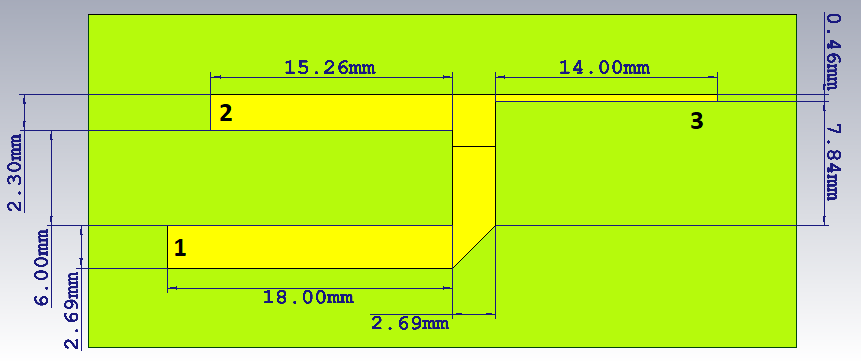
\includegraphics[scale=0.5]{p1_sec2_ustrip}
	\caption{Splitter2 microstrip implementation. }
	\label{fig:p1_sec2_ustrip}
\end{figure}
\newpage
\begin{table} [h]
	\label{tab:p2_sec2DimQWa}
	\caption{Splitter2: quarter-wavelength a dimensions.}
	\centering	
	\begin{tabular}{lccc} 
		\toprule
		& theoretical & optimized &\\
		\midrule 
		W\textsubscript{QWa} 	&	2.44		&	2.17& mm		\\
		L\textsubscript{QWa}	&	16.96		& 	15.42& mm		\\ 
		Z\textsubscript{c,QWa}	&	56.6		& 	60.4& $\Omega$		\\
		\bottomrule
	\end{tabular}	
\end{table}

\begin{table} [h]
	\label{tab:p2sec2DimQWb}
	\caption{Splitter2: quarter-wavelength b dimensions.}
	\centering	
	\begin{tabular}{lccc} 
		\toprule
		& theoretical & optimized &\\
		\midrule 
		W\textsubscript{QWb} 	&	0.613		&0.43& mm		\\
		L\textsubscript{QWb}	&	17.709		& 14.11& mm		\\ 
		Z\textsubscript{c,QWb}	&	105			& 118& $\Omega$		\\
		\bottomrule
	\end{tabular}	
\end{table}

\newpage

\begin{figure}[H] 
	\centering
	\subfloat[][\emph{Modulus}]{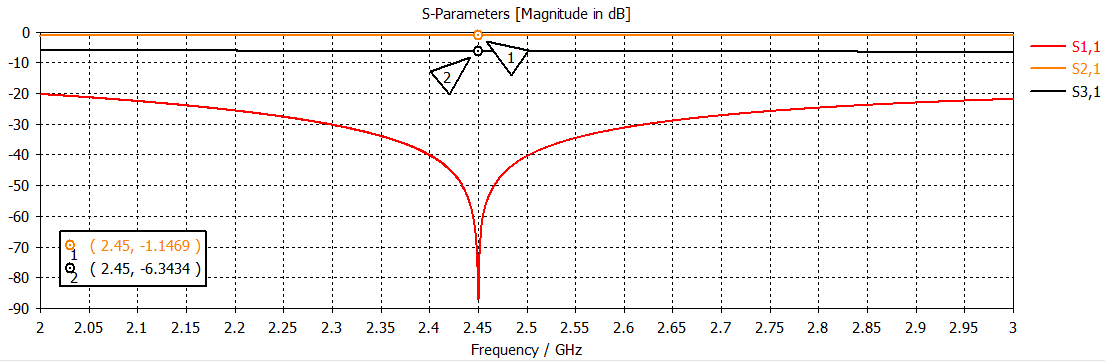
\includegraphics[scale=.6,angle=90]{p1_sec2_Smod}}\quad
	\subfloat[][\emph{Phase}]{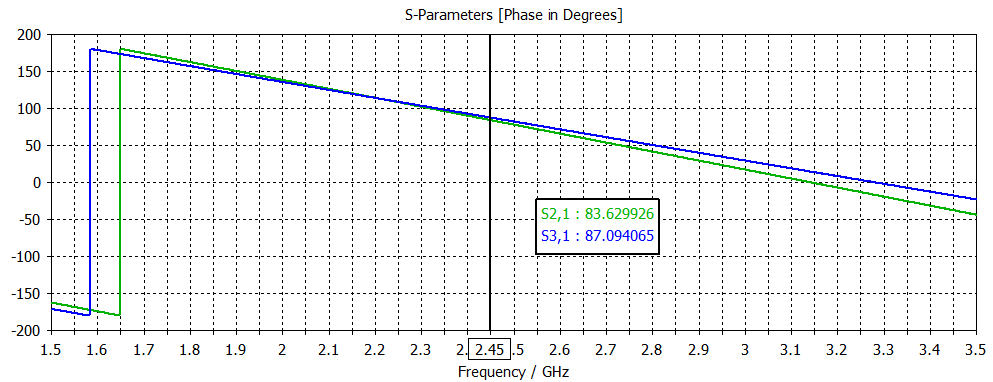
\includegraphics[scale=.6,angle=90]{p1_sec2_Sph}}\\
	\caption{Section 1 most important scattering parameters. As it appears both input matching and even power splitting are accomplished. The tapering value is t=-5.2dB, the phase shift amount to 3.94$^\circ$ (reference impedance 50$\Omega$).}.
	\label{fig:p2_sec1Scatt}
\end{figure}
\newpage
\subsection{Match2 design}

As final design step, another quarter-wavelength transformer is introduced. This element matches splitter2 and splitter3, R\textsubscript{out}=50$\Omega$, output impedance with the radiators' input impedance, equal to Z\textsubscript{in,patch}=120$\Omega$. Using equation (\ref{eq:p1_ZcQW}) we have:
\begin{align}
	Z_{c,M2}&=\sqrt{R_{in,M2}\cdot R_{out,M2}} \notag\\
	&=\sqrt{Z_{out}\cdot Z_{in,patch}} \notag\\
	&=\sqrt{120\Omega \cdot 50\Omega}=77.5\Omega \notag
\end{align}
The conversion from ideal microstrip to layout can be found in table 6, whereas the return loss is shown in figure \ref{fig:p1_M2_Smod}

\begin{table} [H]
	\label{tab:21_DimM2}
	\caption{Match2: microstrip dimensions.}
	\centering	
	\begin{tabular}{lccc} 
		\toprule
		& theoretical 			& optimized &\\
		\midrule 
		W\textsubscript{M2} 	&	1.32		&	1.21	& mm 		\\
		L\textsubscript{M2}		&	17.37		& 	17.37	& mm		\\ 
		Z\textsubscript{c,M2}	&	77.5		& 	80.4	& $\Omega$		\\
		\bottomrule
	\end{tabular}	
\end{table}

\begin{figure}[t] 
	\centering
	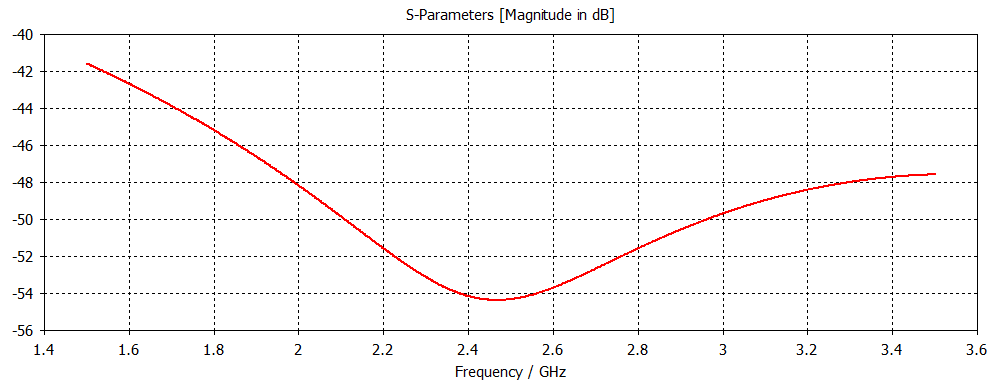
\includegraphics[scale=0.43]{p1_M2_Smod}
	\caption{Match2 return loss (reference impedance 77.5$\Omega$). }
	\label{fig:p1_M2_Smod}
\end{figure}
\newpage
\begin{figure}[H] 
	\centering
	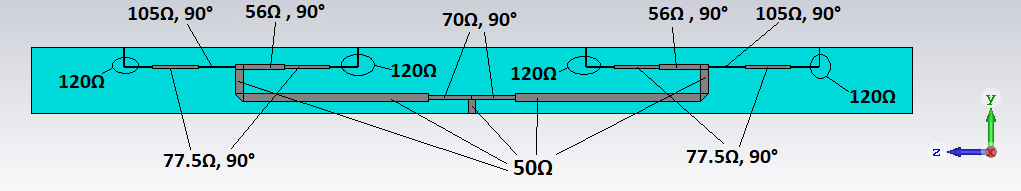
\includegraphics[scale=0.7,angle=90]{p1_bfn_compl_BOXES}
	\caption{Full beam forming network. }
	\label{fig:p1_bfn_compl1}
\end{figure}

\newpage

\subsection{Complete BFN with dimensions}

Now that all the main components have been optimized the following step includes the merging of all the sections as shown if figure \ref{fig:p1_bfn_compl1}.
To connect splitter1 with splitter2 we used a 50$\Omega$ line bent in order to be compliant with the radiators' spacing specification. The bend has been chosen with mitered topology, to reduce parasitics. Furthermore, the 50$\Omega$ and 120$\Omega$ lines parallel to the y axis are kept short to reduce the space occupied by the BFN. Within the following paragraph the performed beam forming network simulation will be presented.

All the beam forming network dimensions are grouped from figure \ref{fig:p1_bfn_quot5} to figure \ref{fig:p1_bfn_quot4}.
\begin{figure}[t] 
	\centering
	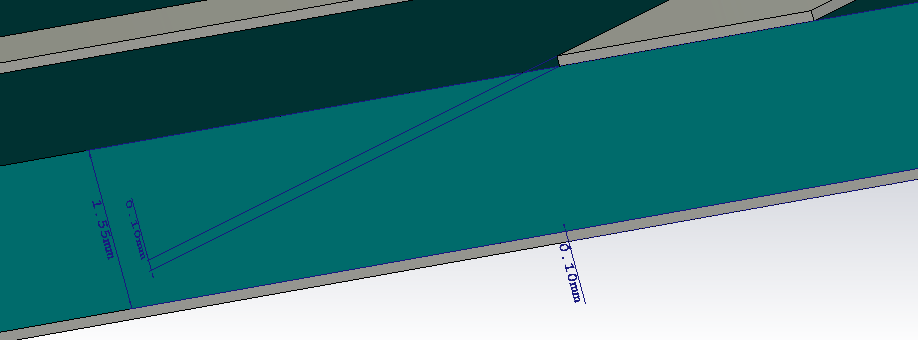
\includegraphics[scale=0.5]{p1_bfn_quot5}
	\caption{Here are highlighted the quoted regions. }
	\label{fig:p1_bfn_quot5}
\end{figure}
\newpage 
\begin{figure}[H] 
	\centering
	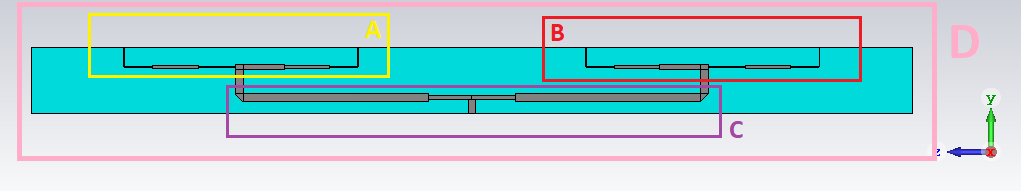
\includegraphics[scale=0.7,angle=90]{p1_bfn_quot0}
	\caption{Here the quoted regions are highlighted. }
	\label{fig:p1_bfn_quot0}
\end{figure}

\begin{figure}[H] 
	\centering
	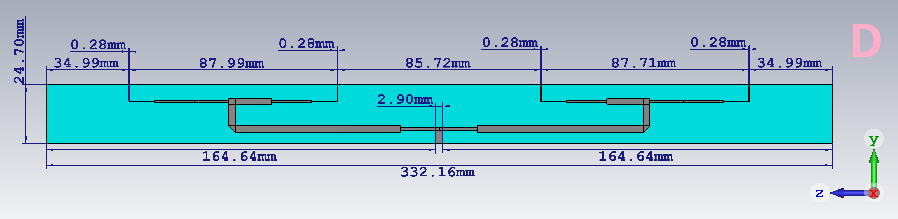
\includegraphics[scale=0.7,angle=90]{p1_bfn_quot1}
	\caption{Quoted BFN: region D. }
	\label{fig:p1_bfn_quot1}
\end{figure}

\begin{figure}[H] 
	\centering
	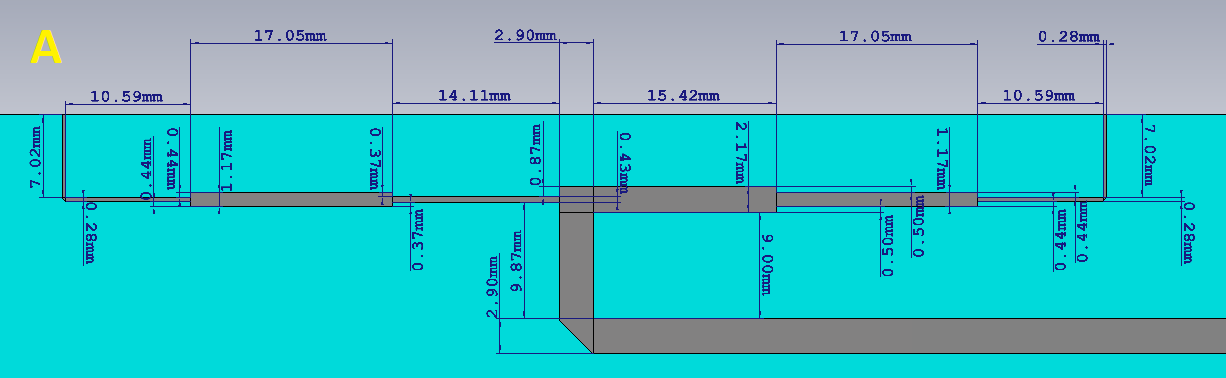
\includegraphics[scale=0.6,angle=90]{p1_bfn_quot2}
	\caption{Quoted BFN: region A. }
	\label{fig:p1_bfn_quot2}
\end{figure}

\begin{figure}[H] 
	\centering
	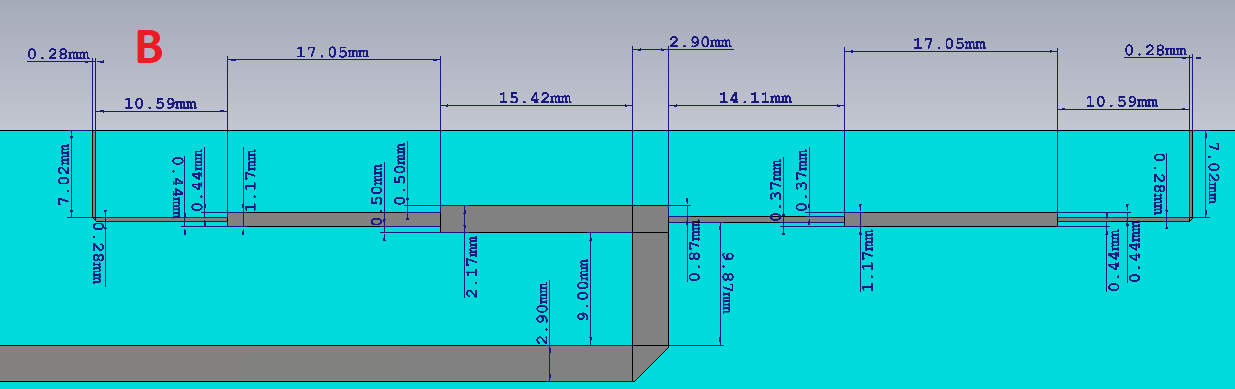
\includegraphics[scale=0.6,angle=90]{p1_bfn_quot3}
	\caption{Quoted BFN: region B. }
	\label{fig:p1_bfn_quot3}
\end{figure}

\begin{figure}[H] 
	\centering
	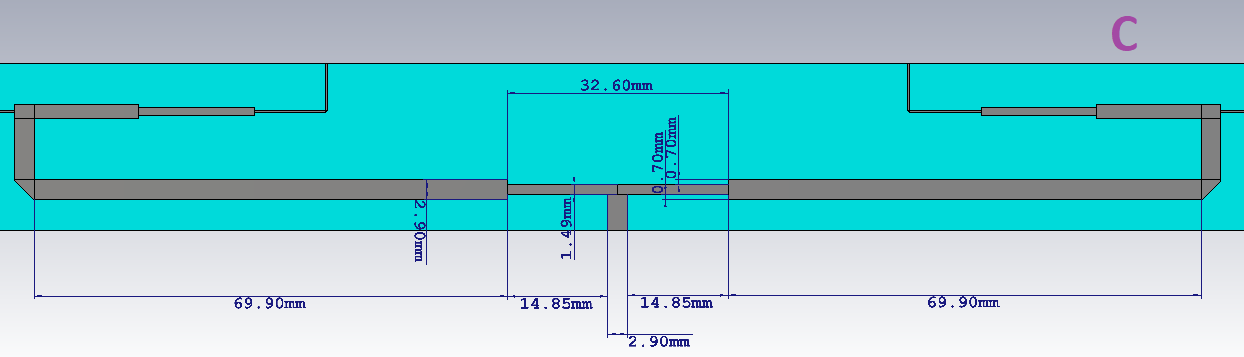
\includegraphics[scale=0.6,angle=90]{p1_bfn_quot4}
	\caption{Quoted BFN: region C. }
	\label{fig:p1_bfn_quot4}
\end{figure}

